\documentclass[
    11pt, % Set the default font size, options include: 8pt, 9pt, 10pt, 11pt, 12pt, 14pt, 17pt, 20pt
    %
    aspectratio=169, % Uncomment to set the aspect ratio to a 16:9 ratio which matches the aspect ratio of 1080p and 4K screens and projectors
]{beamer}

\graphicspath{{Images/}{./}} % Specifies where to look for included images (trailing slash required)
\usepackage{booktabs} % Allows the use of \toprule, \midrule and \bottomrule for better rules in tables

%\usepackage{appendixnumberbeamer} %If you want a separate slide counter for your appendix

%%% Customize Theme %%%%%%%%%%%%%%%%%%%%%%
\usetheme{Madrid} % You can use other themes too, but this changes many things. I've found Madrid to be the best for this color scheme

%fg = font color
%bg = background color

% ! WARNING ! : Many colors are linked to multiple attributes, so changing one color can have unexpected changes!

% If you want to tweak the shading of orange and red, tweak the below 2 lines:t
\definecolor{myRed}{RGB}{120,4,4}
\definecolor{myOrange}{RGB}{227, 125, 0}

% Bottom right hand color
\setbeamercolor*{structure}{bg=myRed!20,fg=myRed!90}

\setbeamercolor*{palette primary}{use=structure,fg=white,bg=structure.fg} %?
\setbeamercolor*{palette secondary}{use=structure,fg=myRed,bg=white}
    %bottom left of footer & bar between title & top bubbles
\setbeamercolor*{palette tertiary}{use=structure,fg=white,bg=myRed} 

\setbeamercolor{frametitle}{bg=myRed!85,fg=white} %title of each slide

\setbeamercolor*{titlelike}{parent=palette primary} %?
%\setbeamercolor{titlelike}{parent=palette primary,fg=structure.fg!50!myRed}

%for miniframe (very top) AND center footer
\setbeamercolor{section in head/foot}{fg=myOrange, bg=white}

%%% Specific Colors %%%
\setbeamercolor{item projected}{bg=myOrange}
\setbeamertemplate{enumerate items}{bg=myOrange}

\setbeamercolor{itemize item}{fg=myOrange}
\setbeamercolor{itemize subitem}{fg=myOrange}

\setbeamercolor{button}{bg=myOrange}

%%% Edits ONLY the TOC slide %%%
\setbeamercolor{section in toc}{fg=black}
\setbeamercolor{subsection in toc}{fg=black}

%%% Block Colors %%%
% Standard block %
    \setbeamercolor{block title}{bg=myOrange, fg=white}
    \setbeamercolor{block body}{bg=myOrange!20}

% Alerted block % If you want to customize it's color
    %\setbeamercolor{block title alerted}{bg=cyan, fg=white}
    %\setbeamercolor{block body alerted}{bg=cyan!10}

% Example block % If you want to customize it's color
    %\setbeamercolor{block title example}{bg=cyan, fg=white}
    %\setbeamercolor{block body example}{bg=cyan!10}

%---------------------------------------------------------
%	SELECT FONT THEME & FONTS
%---------------------------------------------------------
\usefonttheme{default} % Typeset using the default sans serif font
\usepackage{palatino} % Use the Palatino font for serif text
\usepackage[default]{opensans} % Use the Open Sans font for sans serif text
\useinnertheme{circles}

%---------------------------------------------------------
%	SELECT OUTER THEME
%---------------------------------------------------------
% Outer themes change the overall layout of slides, such as: header and footer lines, sidebars and slide titles. Uncomment each theme in turn to see what changes it makes to your presentation.

%\useoutertheme{default}
%
\useoutertheme{miniframes}

%\useoutertheme{infolines}
%\useoutertheme{smoothbars}
%\useoutertheme{sidebar}
%\useoutertheme{split}
%\useoutertheme{shadow}
%\useoutertheme{tree}
%\useoutertheme{smoothtree}

%---------------------------------------------------------
%	PRESENTATION INFORMATION
%---------------------------------------------------------

\title[Middle Footer]{Diachronic Embeddings}
\subtitle{Modelling the semantic change over time}
\author[Left Footer]{Author: Aymane Hachcham}

\institute[]{Department of Statistics \\}
\date[WiSE 2022/23]
%\date[\today]

\logo{
\includegraphics[width=1.5cm]{Images/tu.png}}

%---------------------------------------------------------
%---------------------------------------------------------
%---------------------------------------------------------
\begin{document}

%---------------------------------------------------------
%	TITLE SLIDE
%---------------------------------------------------------
\section{}
\begin{frame}
	\titlepage % Output the title slide, automatically created using the text entered in the PRESENTATION INFORMATION block above
 
\end{frame}

%---------------------------------------------------------
%	TABLE OF CONTENTS SLIDE
%---------------------------------------------------------
% The table of contents outputs the sections and subsections that appear in your presentation, specified with the standard \section and \subsection commands. You may either display all sections and subsections on one slide with \tableofcontents, or display each section at a time on subsequent slides with \tableofcontents[pausesections]. The latter is useful if you want to step through each section and mention what you will discuss.

\begin{frame}
	\frametitle{Table of Contents} % Slide title, remove this command for no title
	
	\tableofcontents % Output the table of contents (all sections on one slide)
	%\tableofcontents[pausesections] % Output the table of contents (break sections up across separate slides)
\end{frame}

%---------------------------------------------------------
%	PRESENTATION BODY SLIDES
%---------------------------------------------------------
\section{Motivation} % Sections are added in order to organize your presentation into discrete blocks, all sections and subsections are automatically output to the table of contents as an overview of the talk but NOT output in the presentation as separate slides

%------------------------------------------------
\begin{frame}
	\frametitle{Diachronic Analysis}
            \begin{itemize}
                \item The term \textbf{Diachronic} refers to the study of how something changes over time. In linguistics,    \textit{Diachronic analysis} is concerned with the way that language changes over time.
                \item It Examines how to following evolves over time:
                 \begin{itemize}
                    \item How forms and meanings of words
                    \item Grammatical structures
                    \item Pronunciation
                \end{itemize}
            \end{itemize}
            
\end{frame}

    \begin{frame}
    \frametitle{Diachronic Sematic Shifts}
    \begin{itemize}
        \item An active research Field.
        \item Research possible because of:\textbf{Existence of large corpora} and \textbf{development of computational semantics}.
    \end{itemize}

    \begin{figure}
        \centering
        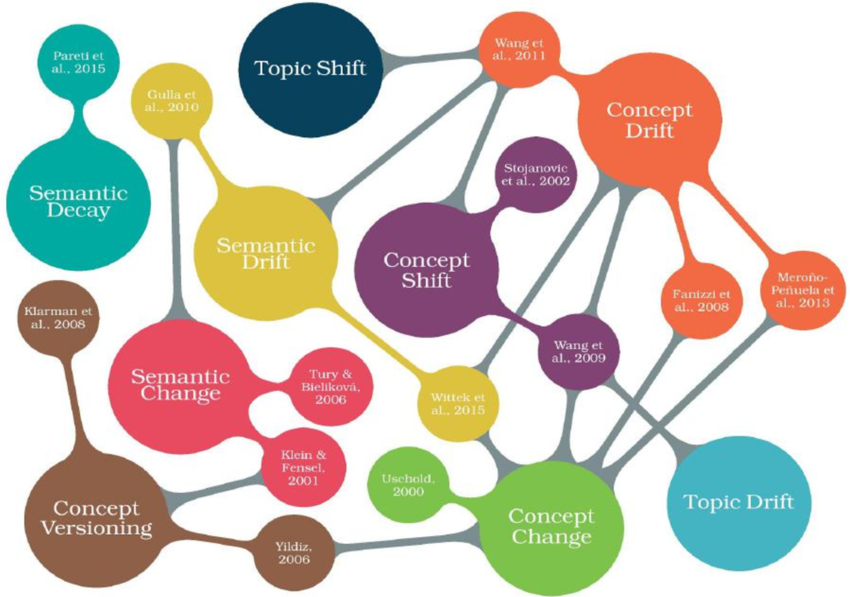
\includegraphics[width=6.5cm]{Images/semantic.png}
        \label{fig:my_label}
    \end{figure}
    
\end{frame}

\begin{frame}
    \frametitle{Diachronic Semantic Shifts}
	% \framesubtitle{Context and Background}
    \begin{exampleblock}{First Research}
        \begin{itemize}
            \item \textit{(Bloomfield 1933)}: "\textit{innovations which change the lexical meaning rather than the grammatical function of a form.}"
            \item \textit{(Bréal, 1899; Stern, 1931; Bloomfield, 1933)}: Found the 9 most prominent categories in semantic shift.
            \item \textit{(Blank and Koch, 1999; Grzega and Schoener, 2007)}: Determined the driving forces for semantic change.
            \item \textit{(Mikolov et al., 2013b)}: Used word embeddings to model Diachronic Semantic change.
        \end{itemize}
    \end{exampleblock}

    
\end{frame}

\begin{frame}
    \frametitle{Diachronic Sematic Shifts}
    \begin{block}{Types of Semantic Shifts}
        Theoretical linguists have identified regularities in language change and have described various types of lexical semantic shifts:
    \begin{itemize}
        \item Narrowing/Broadening the sense 
        \item Positive/Negative connotations
        \item Cultural Changes
    \end{itemize}
    \end{block}
    \underline{Examples}:
    \begin{itemize}
        \item \textit{"mete"} (food, all kinds of food)       \textit{"meat"} (edible flesh)
        \item \textit{"gay"} (joyful, cheerful, sweet) \textit{"gay"} (Homosexual)
        \item \textit{"Iraq"}, \textit{"Syria"} (Cities in Middle East) \textit{"Iraq"}, \textit{"Syria"} (Synonyms of war).
    \end{itemize}
    
\end{frame}

\begin{frame}{Diachronic Sematic Shifts}
    \begin{block}{Drivers}
        The drivers or factors that lead to Sematinc Shifts can be:
        \begin{itemize}
            \item Linguistic
            \item Psychological
            \item Sociocultural
        \end{itemize}
    \end{block}
    
\end{frame}

%------------------------------------------------
\section{Methodology}
%------------------------------------------------
\begin{frame}
    \frametitle{Tasks and Methods}

    \textbf{Objective:}
      Study the evolution in the meanings of these words over time by comparing the representations of their meanings across different periods.
     \begin{block}{Modelling semantic shifts} 
         \begin{itemize}
             \item The research investigates the way in which the meanings of words change over time in a corpus of documents.
             \item The documents are divided into different time periods, and the meanings of target words are analyzed by examining how they are used in context during each time period.
         \end{itemize}
     \end{block}
      
    
\end{frame}

\begin{frame}
    \frametitle{Tasks and Methods}
    
     \begin{block}{Tracing Semantic Shifts} 
         From a collection of corpora $[C_{1},C_{2},...,C_{n} ]$ with periods of time of different granularity ranging from $[1,2,...,n]$, we can trace the words that change in meaning most often.
     \end{block}
     \begin{block}{Other Methods} 
         Other important tasks:
         \begin{itemize}
             \item Quantifying the degree of semantic change of each word in a corpus. 
             \item Detecting whether words undergo semantic change or not in a corpus.
             \item Interpreting the change undergone by a word.
         \end{itemize}
     \end{block}
    
\end{frame}



\begin{frame}
    \frametitle{Tasks and Methods}
    
     \textbf{Two main approaches}
     \begin{block}{Word frequency}
         Analyzing the statistical distribution of words across different time periods. This involved calculating the frequency of words in each time period (Michel et al. 2011)
     \end{block}
     \begin{block}{Word co-occurrences}
         Word collocations, or the words that tend to occur together, can be useful for understanding how the general context of a word changes over time:
         \begin{itemize}
             \item (Hilpert 2006): Compute statistical dependency between pairs of words at different times slices in a corpus.
             \item (Sagi et al. 2009): Words are represented using Singular Value Decomposition on a condensed version of a matrix of co-occurrences.
         \end{itemize}
     \end{block}
    
\end{frame}

\begin{frame}
    \frametitle{Neural word Embeddings}

    Latest research focuses on word embeddings, which are real-valued vectors that represent a word and its usage based on the contexts in which it appears. 
    \begin{figure}
        \centering
        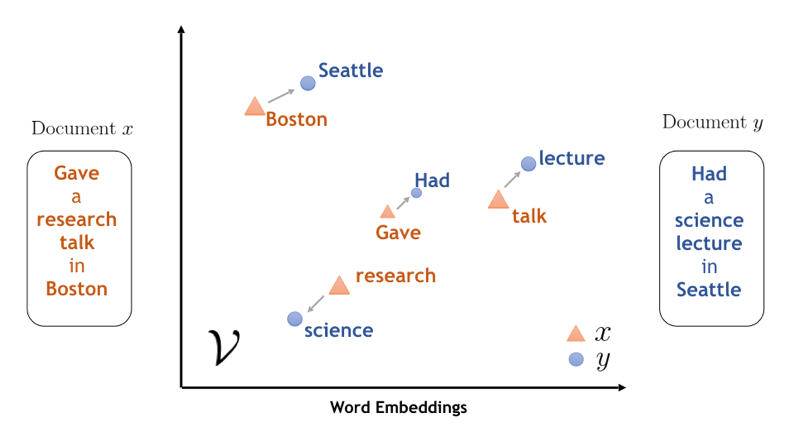
\includegraphics[width=8.5cm]{Images/embeds.png}
        \label{fig:my_label}
    \end{figure}
    
\end{frame}

\begin{frame}
    \frametitle{Neural word Embeddings}

    \textbf{Main idea}:
     Word embeddings are an extension of distributional similarity methods, which are based on the idea that words with similar meanings tend to appear in similar contexts.

     \begin{exampleblock}{Methods for learning word embeddings}
         \begin{itemize}
             \item Word2Vec (Mikolov, Chen, Corrado, and Dean, 2013), which has two algorithms called Continuous Bag of Words (CBOW) and Skip-Gram.
             \item Glove (Pennington, Socher, and Manning, 2014), which is based on the factorization of a word-context co-occurrence matrix.
             \item FastText (Bojanowski, Grave, Joulin, and Mikolov, 2017) is another algorithm for learning word embeddings that handles out-of-vocabulary words.
         \end{itemize}
     \end{exampleblock}
    
\end{frame}

\begin{frame}
    \frametitle{Focus on Word2Vec}

    The Word2Vec framework is made up of two models, called Continuous Bag of Words (CBOW) and Skip-Gram.

    \begin{figure}
        \centering
        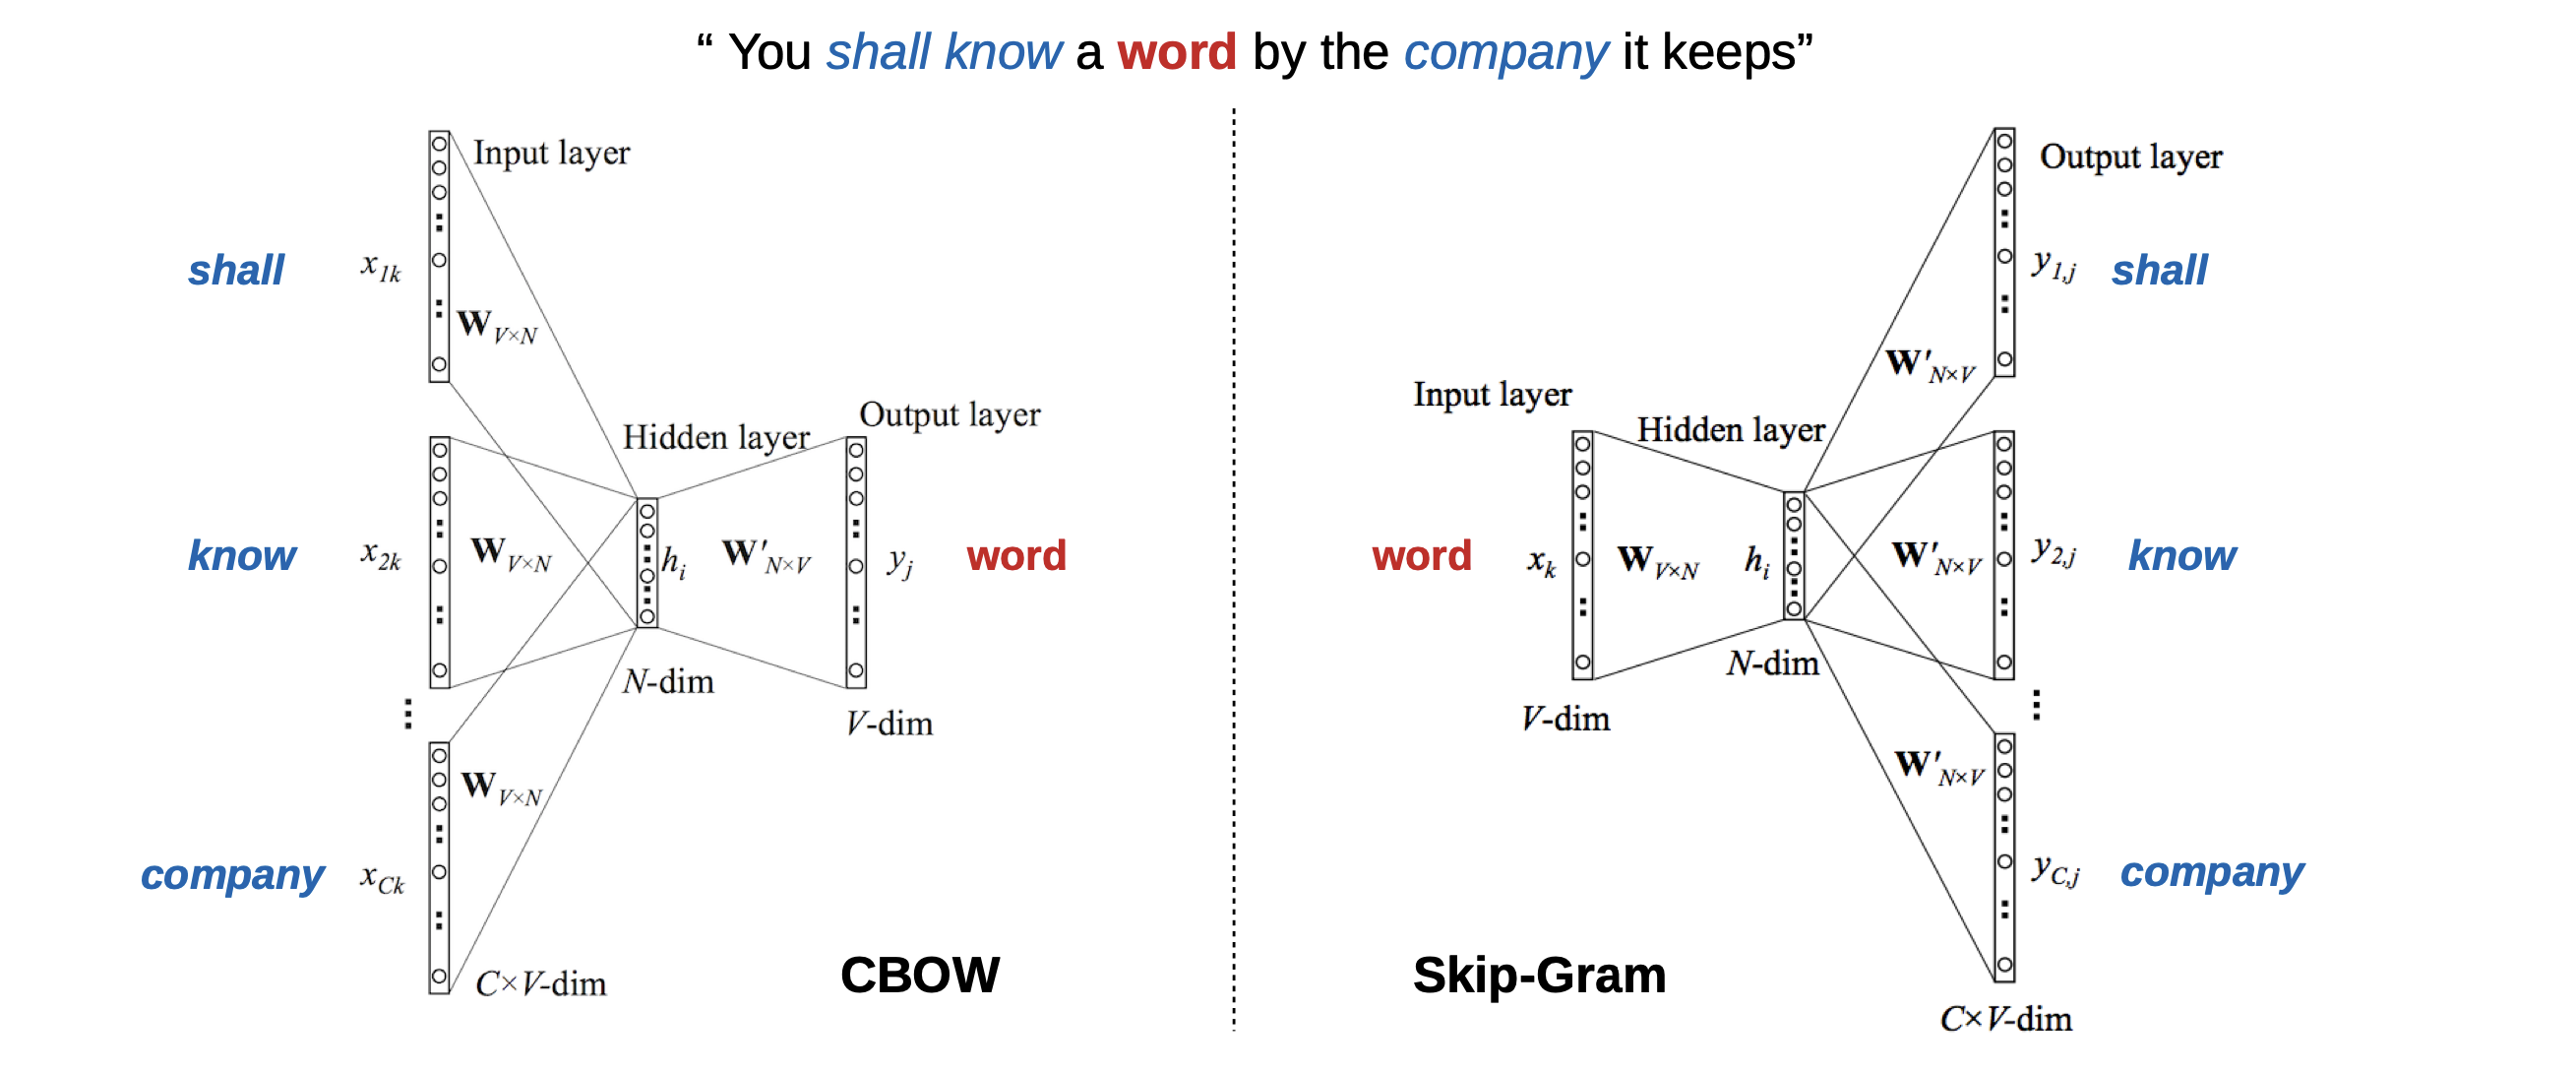
\includegraphics[width=10.5cm]{Images/mod.png}
        \label{fig:my_label}
    \end{figure}
     
\end{frame}

\begin{frame}
    \frametitle{Focus on Word2Vec}

    Continuous Bag of Words (CBOW) and Skip-Gram, are both two-layer neural networks that are designed to learn the linguistic contexts of words and represent them in a vector space.
    \begin{block}{}
        \begin{itemize}
            \item CBOW predicts which word is most likely to appear based on the context in which it appears.
            \item CBOW treats the full context of a word as a single observation.
            \item Skip-Gram uses the network to predict the context words around a given target word.
            \item Skip-Gram treats each context-target pair as a separate observation.
        \end{itemize}
    \end{block}
     
\end{frame}




% \begin{frame}
	
	
% 	Look at the code of this slide to see how columns made this formatting look nice.

% 	\begin{columns}[t] % The "c" option specifies centered vertical alignment while the "t" option is used for top vertical alignment
% 		\begin{column}{0.5\textwidth} % Right column width
%                 \begin{figure}[h!]
%                     \centering
%                     %\caption{Hawkins et al, 2015}
%                     
\includegraphics[angle=0, width=4.5cm]{Hokie2.png}
%                     %\label{Figure 1}
%                 \end{figure}
% 		\end{column}
%   		\begin{column}{0.5\textwidth} % Left column width
%                 \begin{figure}[h!]
%                     \centering
%                     %\caption{Hawkins et al, 2015}
%                     
\includegraphics[angle=0, width=4.5cm]{Hokie2.png}
%                     %\label{Figure 1}
%                 \end{figure}
% 		\end{column}		
% 	\end{columns}
% \end{frame}

%------------------------------------------------
\begin{frame}
	\frametitle{Yet another title}
            You can use bullets too:\newline
            \begin{itemize}
                \item Like this one\newline
                \item \& this one
            \end{itemize}
\end{frame}

%------------------------------------------------
\begin{frame}
\label{Test} %For the link button for the Appendix slide
	\frametitle{A title}

        \begin{itemize}
            \item You can also nest sub-bullets
            \begin{itemize}
                \item Constant
                \item Cubic
                \item Continuous (with slope changes)
                \item Exponential \newline
            \end{itemize}
        \end{itemize}

        \textbf{Below is a button that links to a slide in the appendix}
        
        \begin{center}
            \hyperlink{Figure}{\beamergotobutton{Go to graphs}}    
        \end{center}
\end{frame}

%------------------------------------------------


%------------------------------------------------
\begin{frame}
\label{Test Stat}
	\frametitle{The Test Statistic}
		
        Here is a made up equation:
        $$ \hat{A} = \bar{m}-\hat{m}_S$$ \newline

        Notice how these buttons are centered and evenly spread out:\newline

        \begin{columns}[t] % The "c" option specifies centered vertical alignment while the "t" option is used for top vertical alignment
		\begin{column}{0.25\textwidth} % Right column width
                \hyperlink{Terms}{\beamergotobutton{Go to Terms}}
		\end{column}
  		\begin{column}{0.25\textwidth} % Left column width
                \hyperlink{Definitions}{\beamergotobutton{Go to Definitions}}
		\end{column}
            \begin{column}{0.25\textwidth} % Left column width
                \hyperlink{Theorems}{\beamergotobutton{Go to Theorems}}
		\end{column}
	\end{columns}
        
\end{frame}

%------------------------------------------------
\begin{frame}
	\frametitle{No way, another title!}
            \begin{enumerate}
                \item Instead of bullets, you can index by number too\newline
                \item like this
            \end{enumerate}
\end{frame}

%------------------------------------------------
\section{Testing}

%------------------------------------------------
\begin{frame}
	\frametitle{Second to last title}
    	\begin{block}{Block Title}
    		Block 1
    	\end{block}
    	
    	\begin{exampleblock}{Example Block Title}
    		Block 2
    	\end{exampleblock}
    	
    	\begin{alertblock}{Alert Block Title}
    		Block 3
    	\end{alertblock}
    	
    	\begin{block}{} % Block without title
    		Block without a title
    	\end{block}
\end{frame}

%------------------------------------------------
\section{Conclusion}
%------------------------------------------------
\begin{frame}
	\frametitle{Last title}
		
	Last bit of text

\end{frame}

%---------------------------------------------------------
%	CLOSING SLIDE
%---------------------------------------------------------

% To remove miniframe from top
\appendix
\setbeamertemplate{headline}{}
\addtobeamertemplate{frametitle}{\vspace*{-\headheight}}{}

\begin{frame}[noframenumbering] %So the end and appendix slides don't contribute to the page count
%[plain] % The optional argument 'plain' hides the headline and footline
	%\frametitle{Questions?}

	\begin{center}
            {\LARGE Questions?}
	\end{center}
 
\end{frame}
%---------------------------------------------------------

%------------------------------------------------
\begin{frame}[noframenumbering]
\label{Figure}
	\frametitle{Appendix - A figure}
        \hyperlink{Test}{\beamerreturnbutton{Return to presentation}}
        
        \begin{figure}[h!]
            \centering
            %\caption{}
            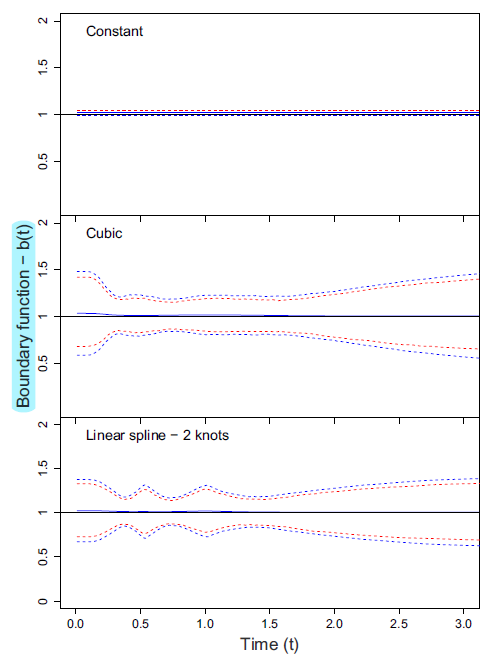
\includegraphics[angle=0, width=5cm]{Newey et al Graph.png}
            %\label{fig}
        \end{figure}
\end{frame}

%------------------------------------------------
\begin{frame}[noframenumbering]
\label{Terms}
	\frametitle{Appendix - Terms}

        \begin{columns}[t] % The "c" option specifies centered vertical alignment while the "t" option is used for top vertical alignment
		\begin{column}{0.5\textwidth} % Right column width
                Some Estimators:
                \begin{itemize}
                    \item Drift: $\hat{\delta}$
                    \item Boundary: $\hat{b}(t)$
                \end{itemize}
		\end{column}
  		\begin{column}{0.5\textwidth} % Left column width
                Some Variables:
                \begin{itemize}
                    \item $\hat{V}$
                    \item $\hat{m}_S$
                    \item $\bar{m}$
                    \item $m_J(\tau)$\newline\newline
                \end{itemize}
		\end{column}
	\end{columns}
        \hyperlink{Test Stat}{\beamerreturnbutton{Return to presentation}}        
\end{frame}

%------------------------------------------------
\begin{frame}[noframenumbering]
\label{Definitions}
	\frametitle{Appendix - Definitions}
         \begin{enumerate}
             \item A definition \newline
         \end{enumerate}
         
        \hyperlink{Test Stat}{\beamerreturnbutton{Return to presentation}}
\end{frame}

%------------------------------------------------
\begin{frame}[noframenumbering]
\label{Theorems}
	\frametitle{Appendix - Theorems}
         \begin{enumerate}
             \item A theorem\newline
         \end{enumerate}
         
        \hyperlink{Test Stat}{\beamerreturnbutton{Return to presentation}}        
\end{frame}

\end{document} 